\documentclass[12pt]{article}
\usepackage[utf8]{inputenc}
\usepackage{amsmath,amsthm,amsfonts,amssymb}
\usepackage{tikz}
\usepackage{subfig}
\usepackage[english]{babel}
\usepackage{capt-of}
\newtheorem{theorem}{Theorem}
\usetikzlibrary{calc}
\usetikzlibrary{shapes}
\usepackage{hyperref}
%might be unnecessary
\usepackage{doi}

%bibliography CMDS

%\usepackage{cite}
%\usepackage[style=alphabetic]{biblatex}
%\bibliographystyle{plain}

%\usepackage[style=alphabetic]{biblatex}

\usepackage[backend=biber,style=alphabetic]{biblatex}
%\usepackage[backend=bibtex,style=alphabetic]{biblatex}
\addbibresource{bibb.bib}

%%% With amsthm package, creates environments for nicely formatted,
%%% labeled, and numbered propositions, etc.
\theoremstyle{plain}
\newtheorem{thm}{Theorem}
\newtheorem{lemma}[thm]{Lemma}
\newtheorem{prop}[thm]{Proposition}
\newtheorem{conj}[thm]{Conjecture}
\newtheorem{cor}[thm]{Corollary}
\newtheorem{claim}[thm]{Claim}
\newtheorem{fact}[thm]{Fact}

\theoremstyle{definition}
\newtheorem{eg}[thm]{Example}
\newtheorem{defn}[thm]{Definition}
\newtheorem{rem}[thm]{Remark}
\newtheorem{observ}[thm]{Observation}
\newtheorem{open}[thm]{Open Problem}
\newtheorem{prob.}[thm]{Problem}
\newtheorem{quest}[thm]{Question}

% I used these for making definitions and theorems, not what is above
\theoremstyle{remark}
\newtheorem{remark}[thm]{Remark}
\newtheorem{note}[thm]{Note}
\theoremstyle{definition}
\newtheorem{definition}{Definition}[section]
\newtheorem{exmp}{Example}[section]

%custom commands

% blank cell
\newcommand{\cell}[4]{ \draw[thick] ( #1 , #2 ) rectangle ( #3 , #4 );}

% open cell 
\newcommand{\cellopen}[4]{ \draw[thick] ( #1 , #2 ) rectangle ( #3 , #4 ); \node[shape=circle,draw=red,fill=red, inner sep=0pt,minimum size=3pt] (A) at ( #1 * 0.5 + #3 * 0.5 , #2 * 0.5 + #4 * 0.5 ){};}

% /
\newcommand{\cellA}[4]{ \draw[thick] ( #1 , #2 ) rectangle ( #3 , #4 ); \draw[red, thick] (#3 * 0.5 + #1 * 0.5 , #2) -- (#3, #4 * 0.5 + #2 * 0.5);}

% \
\newcommand{\cellB}[4]{ \draw[thick] ( #1 , #2 ) rectangle ( #3 , #4 ); \draw[red, thick] (#3 * 0.5 + #1 * 0.5 , #2) -- (#1, #4 * 0.5 + #2 * 0.5);}

% /
\newcommand{\cellC}[4]{ \draw[thick] ( #1 , #2 ) rectangle ( #3 , #4 ); \draw[red, thick] (#3 * 0.5 + #1 * 0.5 , #4) -- (#1, #4 * 0.5 + #2 * 0.5);}

% L
\newcommand{\cellD}[4]{ \draw[thick] ( #1 , #2 ) rectangle ( #3 , #4 ); \draw[red, thick] (#3 * 0.5 + #1 * 0.5 , #4) -- (#3, #4 * 0.5 + #2 * 0.5);}

% |
\newcommand{\cellE}[4]{ \draw[thick] ( #1 , #2 ) rectangle ( #3 , #4 ); \draw[red, thick] (#3 * 0.5 + #1 * 0.5 , #2) -- (#3 * 0.5 + #1 * 0.5 , #4);}

% -
\newcommand{\cellF}[4]{ \draw[thick] ( #1 , #2 ) rectangle ( #3 , #4 ); \draw[red, thick] (#3, #4 * 0.5 + #2 * 0.5) -- (#1, #4 * 0.5 + #2 * 0.5);}

\newcommand{\cellAf}[4]{\filldraw[gray!40] ( #1 , #2 ) rectangle ( #3 , #4 ); \draw[thick] ( #1 , #2 ) rectangle ( #3 , #4 ); \draw[red, thick] (#3 * 0.5 + #1 * 0.5 , #2) -- (#3, #4 * 0.5 + #2 * 0.5);}

% \
\newcommand{\cellBf}[4]{\filldraw[gray!40] ( #1 , #2 ) rectangle ( #3 , #4 ); \draw[thick] ( #1 , #2 ) rectangle ( #3 , #4 ); \draw[red, thick] (#3 * 0.5 + #1 * 0.5 , #2) -- (#1, #4 * 0.5 + #2 * 0.5);}

% /
\newcommand{\cellCf}[4]{\filldraw[gray!40] ( #1 , #2 ) rectangle ( #3 , #4 ); \draw[thick] ( #1 , #2 ) rectangle ( #3 , #4 ); \draw[red, thick] (#3 * 0.5 + #1 * 0.5 , #4) -- (#1, #4 * 0.5 + #2 * 0.5);}

% L
\newcommand{\cellDf}[4]{\filldraw[gray!40] ( #1 , #2 ) rectangle ( #3 , #4 ); \draw[thick] ( #1 , #2 ) rectangle ( #3 , #4 ); \draw[red, thick] (#3 * 0.5 + #1 * 0.5 , #4) -- (#3, #4 * 0.5 + #2 * 0.5);}

% |
\newcommand{\cellEf}[4]{\filldraw[gray!40] ( #1 , #2 ) rectangle ( #3 , #4 ); \draw[thick] ( #1 , #2 ) rectangle ( #3 , #4 ); \draw[red, thick] (#3 * 0.5 + #1 * 0.5 , #2) -- (#3 * 0.5 + #1 * 0.5 , #4);}

% -
\newcommand{\cellFf}[4]{\filldraw[gray!40] ( #1 , #2 ) rectangle ( #3 , #4 ); \draw[thick] ( #1 , #2 ) rectangle ( #3 , #4 ); \draw[red, thick] (#3, #4 * 0.5 + #2 * 0.5) -- (#1, #4 * 0.5 + #2 * 0.5);}

\usepackage[margin=1in]{geometry}


%doc info
\title{Mosaics}
\author{Jack Hanke}
\date{\today}

\begin{document}

\begin{center}
    \Large
    \textbf{Mosaics}
    
    \vspace{0.4cm}
    \large
    
    Jack Hanke   
    \vspace{0.4cm}
    
    \today
    \vspace{0.4cm}    
\end{center}

\section{Introduction}

Consider \cite{oeis} \cite{Hong_2018} \cite{10.5555/1717824} \cite{Bna2006AWT} the following $6$ unit squares with markings on them.

%figure of tiles (colored marknigs!)
\begin{center}
    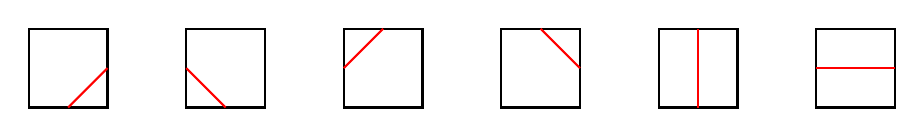
\begin{tikzpicture}
    \cellA{0}{0}{1}{1}
    \cellB{2}{0}{3}{1}
    \cellC{4}{0}{5}{1}
    \cellD{6}{0}{7}{1}
    \cellE{8}{0}{9}{1}
    \cellF{10}{0}{11}{1}    
    \end{tikzpicture}
\end{center}

Call these squares \textit{tiles}. 

\begin{definition}
An $(n,m)$-\textit{mosaic} is a rectangular grid made up of tiles.
\end{definition}

\begin{exmp}
An example of a $(7,5)$-mosaic:
\begin{center}
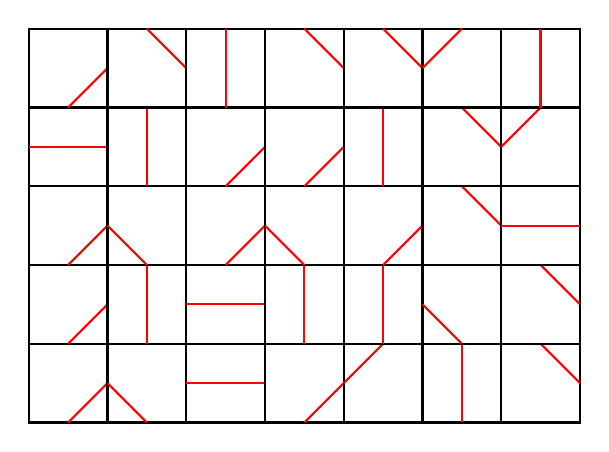
\begin{tikzpicture}
% row1
\cellA{0}{0}{1}{1}
\cellB{1}{0}{2}{1}
\cellF{2}{0}{3}{1}
\cellA{3}{0}{4}{1}
\cellC{4}{0}{5}{1}
\cellE{5}{0}{6}{1}
\cellD{6}{0}{7}{1}
% row2
\cellA{0}{1}{1}{2}
\cellE{1}{1}{2}{2}
\cellF{2}{1}{3}{2}
\cellE{3}{1}{4}{2}
\cellE{4}{1}{5}{2}
\cellB{5}{1}{6}{2}
\cellD{6}{1}{7}{2}
% row3
\cellA{0}{2}{1}{3}
\cellB{1}{2}{2}{3}
\cellA{2}{2}{3}{3}
\cellB{3}{2}{4}{3}
\cellA{4}{2}{5}{3}
\cellD{5}{2}{6}{3}
\cellF{6}{2}{7}{3}
% row4
\cellF{0}{3}{1}{4}
\cellE{1}{3}{2}{4}
\cellA{2}{3}{3}{4}
\cellA{3}{3}{4}{4}
\cellE{4}{3}{5}{4}
\cellD{5}{3}{6}{4}
\cellC{6}{3}{7}{4}
% row5
\cellA{0}{4}{1}{5}
\cellD{1}{4}{2}{5}
\cellE{2}{4}{3}{5}
\cellD{3}{4}{4}{5}
\cellD{4}{4}{5}{5}
\cellC{5}{4}{6}{5}
\cellE{6}{4}{7}{5}
\end{tikzpicture}
\end{center}
\end{exmp}

Clearly there are $6^{nm}$ possible mosaics. Which of these mosaics contain self-avoiding polygons?

%example of a mosaic with an enclosed region
\begin{exmp}
An example of a $(7,5)$-mosaic with a self-avoiding polygon:
\begin{center}
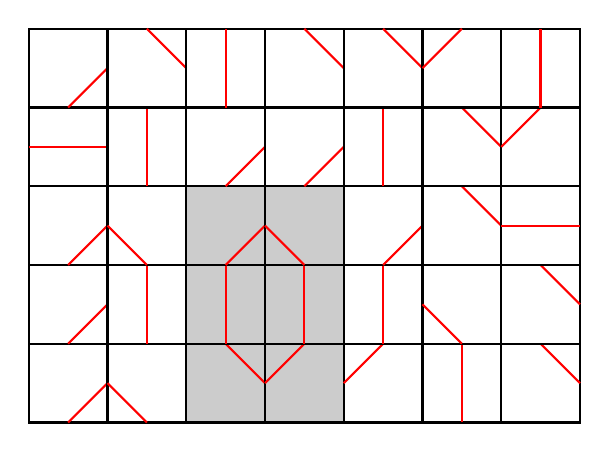
\begin{tikzpicture}
% row1
\cellA{0}{0}{1}{1}
\cellB{1}{0}{2}{1}
\cellDf{2}{0}{3}{1}
\cellCf{3}{0}{4}{1}
\cellC{4}{0}{5}{1}
\cellE{5}{0}{6}{1}
\cellD{6}{0}{7}{1}
% row2
\cellA{0}{1}{1}{2}
\cellE{1}{1}{2}{2}
\cellEf{2}{1}{3}{2}
\cellEf{3}{1}{4}{2}
\cellE{4}{1}{5}{2}
\cellB{5}{1}{6}{2}
\cellD{6}{1}{7}{2}
% row3
\cellA{0}{2}{1}{3}
\cellB{1}{2}{2}{3}
\cellAf{2}{2}{3}{3}
\cellBf{3}{2}{4}{3}
\cellA{4}{2}{5}{3}
\cellD{5}{2}{6}{3}
\cellF{6}{2}{7}{3}
% row4
\cellF{0}{3}{1}{4}
\cellE{1}{3}{2}{4}
\cellA{2}{3}{3}{4}
\cellA{3}{3}{4}{4}
\cellE{4}{3}{5}{4}
\cellD{5}{3}{6}{4}
\cellC{6}{3}{7}{4}
% row5
\cellA{0}{4}{1}{5}
\cellD{1}{4}{2}{5}
\cellE{2}{4}{3}{5}
\cellD{3}{4}{4}{5}
\cellD{4}{4}{5}{5}
\cellC{5}{4}{6}{5}
\cellE{6}{4}{7}{5}
\end{tikzpicture}
\end{center}
\end{exmp}

Let $t_{n,m}$ be the number of mosaics that have at least one self avoiding polygon or SAP. From the fact that the smallest SAP is

\begin{center}
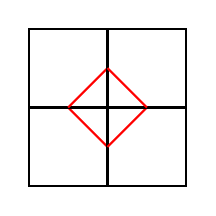
\begin{tikzpicture}

% row1
\cellD{0}{0}{1}{1}
\cellC{1}{0}{2}{1}
% row2
\cellA{0}{1}{1}{2}
\cellB{1}{1}{2}{2}
\end{tikzpicture}
\end{center}

we have that $t_{n,1}=t_{1,m}=0$, and $t_{2,2} = 1$. What else can be said?

\begin{theorem}\label{thm: m=2 case}
Setting $m=2$ gives
\begin{equation}
    \sum_{n \geq 2}t_{n,2}x^n = \frac{x^2}{(1-36x)(1-37x+37x^2)}.
\end{equation}
This can be solved for $n \geq 2$ to give
\begin{equation}
     t_{n,2}= 6^{2n} - \frac{1}{\beta-\alpha}((36\beta-35)\beta^{-n+1} - (36\alpha - 35)\alpha^{-n+1})
\end{equation}

where $\alpha = \frac{1}{2} + \frac{1}{2}\sqrt{\frac{33}{37}}$ and $\beta = \frac{1}{2} - \frac{1}{2}\sqrt{\frac{33}{37}}$.
\end{theorem}

\begin{proof}
We prove that $t_{n,2}$ has
$$t_{n,2} = 36t_{n-1,2} + \sum_{i=2}^{n}(6^{2(n-i)}-t_{n-i,2}).$$

Split $t_{n,2}$ into $S$ and $S^c$. $S$ contains the mosaics that have $1$ SAP only, and the SAP contains the left-most two cells. This means $S^c$ contains all mosaics that contain multiple SAPs and mosaics that contain only $1$ SAP, but that does not contain the two left-most cells.

The subset $S$ can be split further by the length of each SAP $i$. 

\begin{center}
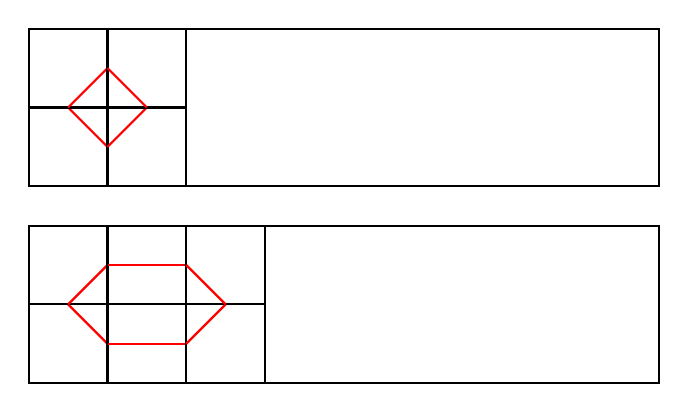
\begin{tikzpicture}
\draw[thick] ( 0 , 0 ) rectangle ( 8 , 2 );
% row1
\cellD{0}{0}{1}{1}
\cellC{1}{0}{2}{1}
% row2
\cellA{0}{1}{1}{2}
\cellB{1}{1}{2}{2}

\draw[thick] ( 0 , -2.5 ) rectangle ( 8 , -0.5 );
% row1
\cellD{0}{-2.5}{1}{-1.5}
\cellF{1}{-2.5}{2}{-1.5}
\cellC{2}{-2.5}{3}{-1.5}
% row2
\cellA{0}{-1.5}{1}{-0.5}
\cellF{1}{-1.5}{2}{-0.5}
\cellB{2}{-1.5}{3}{-0.5}

\end{tikzpicture}
\captionof{figure}{Members of $S$ of lengths $i=2$ and $i=3$}\label{fig: S breakdown}
\end{center}

As $S$ counts the number of mosaics that only contain $1$ SAP, the blank space in Figure \ref{fig: S breakdown} must have no SAPs. The number of mosaics that have no SAPs is $6^{2(n-i)}-t_{n-i,2}$. As a SAP's width can range from $2$ to $n$, we have $|S| = \sum_{i=2}^{n}(6^{2(n-i)}-t_{n-i,2}) = \sum_{i=0}^{n-2}(6^{2(n-i)}-t_{n-i,2})$

Now consider $S^c$. The mosaics that belong to this set can be represented by the following diagram,

\begin{center}
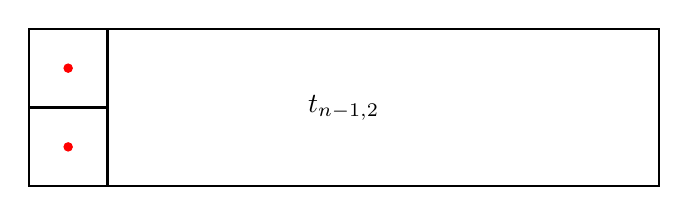
\begin{tikzpicture}
\draw[thick] ( 0 , 0 ) rectangle ( 8 , 2 );
% row1
\cellopen{0}{0}{1}{1}
% row2
\cellopen{0}{1}{1}{2}
% text
\node[shape=circle,draw=white,fill=white, inner sep=0pt,minimum size=0pt] (A) at ( 4 , 1 ){$t_{n-1,2}$};
\end{tikzpicture}
\captionof{figure}{Representation of $S^c$}\label{fig: Sc breakdown}
\end{center}

where the red dot in the left most cells indicate any marking. For this paper, we will refer to a cell that can have any marking as an \textit{open}. We can conclude that $|S^c| = 6^{2}t_{n-1,2}$. Combining $S$ and $S^c$ gives the recurrence relation. Standard techniques then give the generating function and formula.
\end{proof}

\begin{theorem}\label{thm: m=3 case}
Setting $m=3$ gives
\begin{equation}
    \sum_{n \geq 2}t_{n,3}x^n = \frac{(73-414x)x^2}{(1-216x)(1-228x+2699x^2-7758x^3)}
\end{equation}
\end{theorem}

\begin{proof}
Similarly to $t_{n,2}$, we prove a recurrence relation. This time, we prove
$$t_{3,n} = 6^3 t_{n-1,3} + \sum_{i = 0}^{n}(6^{3(n-i)} - t_{n-i,3})f_{i,3}$$
where $f_{n,m}$ is the number of mosaics in an $n \times m$ grid  that contain just one SAP that is $n$ wide and $m$ tall. 

EXAMPLE FIGURE %caption: a mosaic that is counted in f_{7,5}

Notice that $f_{n,2} = 1$ for $n \geq 2$, which is why this 'weight' factor does not appear in the proof of Theorem \ref{thm: m=2 case}. It can be shown that 
$$F_3(x) = \sum_{n \geq 2} f_{n,3}x^n = \frac{73 - 414x}{1-12x+43x^2},$$

and similar techniques prove the generating function.

PROOF OF F RECURRENCE RELATION

\end{proof}

\begin{theorem}
Setting $m=4$ gives
\begin{equation}
    \sum_{n \geq 2}t_{n,4}x^n = ?
\end{equation}
\end{theorem}

%\newpage

%\bibliography{bibtex}{}
\printbibliography


\end{document}